\chapter{Aplicações e resultados\label{chap:aplicacoes}}

Este capítulo apresenta um exemplo básico de utilização do \frame, apresentando as funções principais para para geração de modelos (.inp) e para simulação no ABAQUS, chamada do ABAQUS, pós-processamento e visualização dos resultados. Será apresentados tanto os resultados obtidos com a simulação quanto os códigos básicos utilizados geração desses resultados, bem como trechos des código demonstrando a forma de utilização das principais funcionalidades implementadas.

Embora não haja restrições do \frame\ quanto ao perfil da batimetria, este exemplo será um caso de uma batimetria simples, uma vez que o intúito é apresentar modelo cujos resultados (mais especificamente, os valores das frequências obtidas pela análise modal no ABAQUS) podem validades com os resultados previstos (calculados pela \fatfree).
Vale salientar que os dados utilizados são de domínio público ou fictícios, mas não representam um caso real, até porque que esse tipo de dado é mantido sob sigilo devido a aspectos relacionados à segurança, competitividade tecnológica e propriedade intelectual das empresas do setor.


\section{Exemplo: análise de vida a fadiga de um pequeno trecho de duto\label{sec:model-exemplo}}


O modelo consiste um pequeno trecho de duto com comprimento total de 80~m com um vão de 16~m, cercado por um trecho de solo (ombros) de 32~m de cada lado. As principais Característica geométricas e físicas do duto estão apresentadas na \autoref{tab:propriedades}.

\begin{table}[ht]
	\renewcommand{\arraystretch}{1.2}
		\small
		\centering
		\caption{\label{tab:propriedades} Principais propriedades geométricas do duto}
		\begin{tabular}{lcr}
			\toprule
			Característica & Unidade & Valor\\
			\midrule
			Comprimento do duto &  m & 80\\
			Diâmetro externo &  in & 10,75\\
			Espessura nominal &  in & 0,50\\
			Espessura revestimento &  mm & 2,7\\
			Densidade aço & kg/m$^3$ & 7850\\
			Densidade do revestimento & kg/m$^3$ & 923\\
			Densidade do conteúdo & kg/m$^3$ & 200\\
			Módulo de Elasticidade & Pa & 2,07 $\times 10^{11}$\\
			Limite de Escoamento aço (API 5L-X60) & Pa & 4,14 $\times 10^8$\\
			Comprimento dos elementos (MEF) & m & 0,25\\
			\bottomrule
		\end{tabular}
\end{table}

Tomando partido de uma das funções gráficas, podemos visualizar essa batimetria gerando um gráfico com o perfil. O código para geração dessa figura está na \autoref{code:perfil-da-batimetria}.


\begin{figure}
\caption{Código para geração de \autoref{fig:ex_perfil_da_batimetria} com o perfil da batimetria}\label{code:perfil-da-batimetria}
\begin{pythoncode}
from integrispan.model_generator.model_generator import load_json
from integrispan.plots import plots
model = load_json("inputs.json")
bathymetry_plot = plots.bathymetry(model.bat)
bathymetry_plot.save()
\end{pythoncode}
\end{figure}


Na linha 3 do código exibido na \autoref{code:perfil-da-batimetria}, os dados contidos no arquivo de entrada (\texttt{inputs.json}) são carregados e ficam armazenados em uma instância da classe \texttt{Model}. Na linha 4 é criado o gráfico do perfil de batimetria, que por sua vez é uma instância da classe \texttt{Plot}, e na linha 5 ele é salvo em um arquivo HTML. A \autoref{fig:ex_perfil_da_batimetria} apresenta o resultado.

\begin{figure}[!ht]
    \centering
    \caption{Perfil do modelo.}\label{fig:ex_perfil_da_batimetria}
    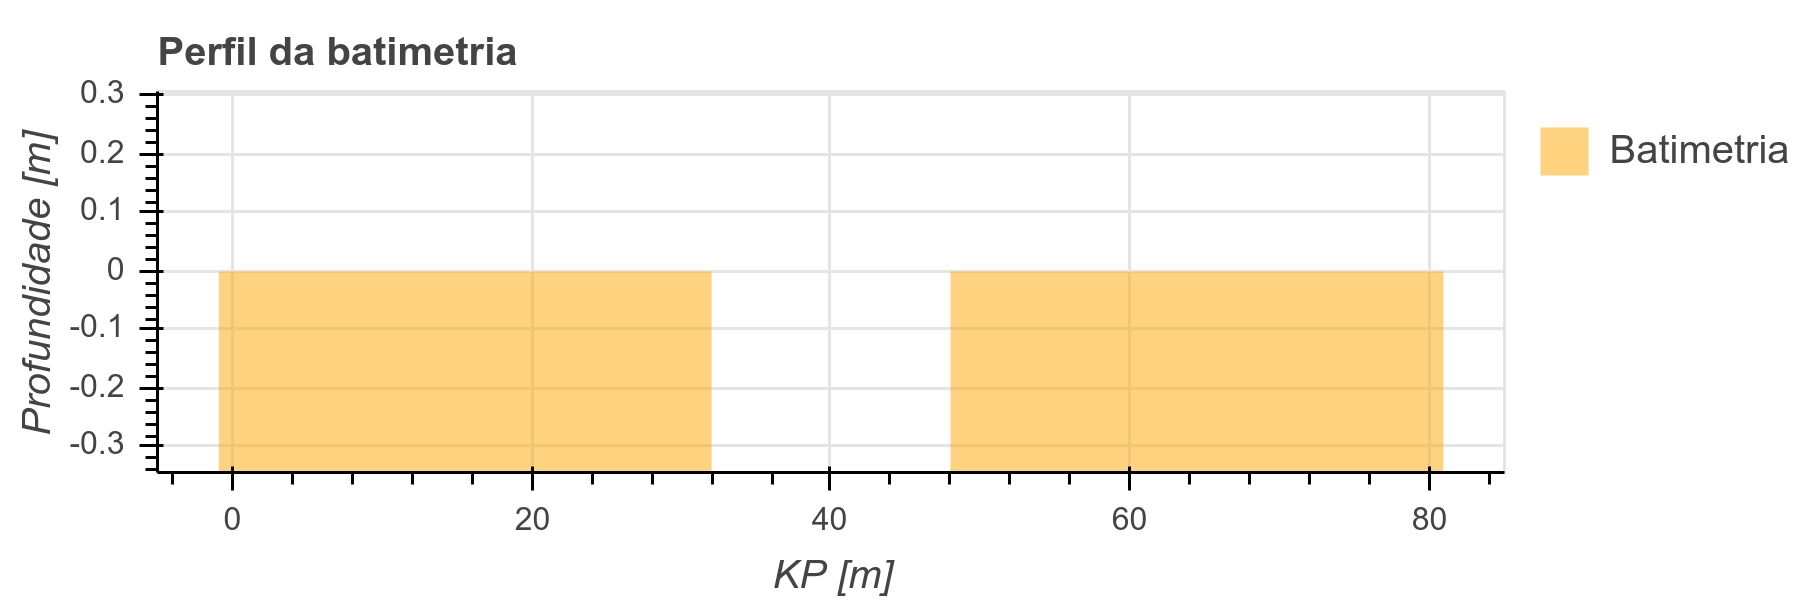
\includegraphics[width=\textwidth]{imagens/ex_perfil_da_batimetriat.png}
    \fonte{Autor (2020)}
\end{figure}

A simulação realizada tem a seguinte sequência de passos de carga:

\begin{enumerate}
	\item Aplica-se o peso do duto vazio;
	\item Aplica-se a pressão externa;
	\item Aplica-se a tração de lançamento;
	\item Aplicas-se o deslocamento vertical e assenta-se o duto;
	\item Restaura-se o atrito axial;
	\item Ativa-se as molas;
	\item Remove a tração de lançamento;
	\item Aplica-se a pressão do teste hidrostático;
	\item Remove-se a pressão do teste hidrostático;
	\item Aplica-se a pressão operacional;
	\item Obtém-se os modos de vibração (análise modal).
\end{enumerate}

Os valores dos carregamentos estão presentes na \autoref{tab:carregamentos}.

\begin{table}[h]
	\renewcommand{\arraystretch}{1.2}
	\small
	\centering
	\caption{\label{tab:carregamentos} Carregamentos do duto.}
	\begin{tabular}{lcr}
		\toprule
		Característica & Unidade & Valor\\
		\midrule
		Pressão externa & kgf/cm$^2$ & 160\\
		Coeficiente de atrito transversal & & 0,8\\
		Coeficiente de atrito longitudinal & & 0,6\\
		Tração Residual de Lançamento & kN & 60\\
		Pressão do teste hidrostático & kgf/cm$^2$ & 160\\ % TODO
		Pressão operacional & kgf/cm$^2$ & 160\\ % TODO
		\bottomrule
	\end{tabular}
\end{table}

A geração dos arquivos para simulação no ABAQUS conteúdo as instruções para toda essa sequência de passo é feita usando o método \texttt{write\_inps}: \texttt{model.write\_inps()}.
Isso deve gerar dois arquivos dentro de um diretório chamado \texttt{exemplo}: o arquivo principal \texttt{exemplo.inp}, e \texttt{bt\_exemplo.inp}, com o definição do perfil de batimetria. \par

O método \texttt{run\_abaqus} do objeto \texttt{model} é responsável por executar a chamada do ABAQUS de maneira programática para iniciar a simulação.
Nesse método, ocorre a leitura do arquivo de log da simulação e o seu conteúdo é exibido na tela do console num intervalo de 5~s.

No caso de haver a colocação de suportes durante, a simulação é executada em duas partes: a primeira com os passos de carga anteriores a passo da colocação dos suportes, e a segunda com o passo da colação dos suportes e os passos de carga seguintes.

Segundo o ítem 6.7.4 da \dnvf105, a análise de elementos finitos com para um único vão com força axial efetiva igual a zero e $L / D_s \approx 60$, as frequências naturais de \textit{in-line} e \textit{cross-flow} e as faixas de tensão devem mostram valores semelhantes com uma margem de $\pm 5\%$.

{\large EM ANDAMENTO...}